\documentclass[apuntes]{subfiles}

\begin{document}

\section{Estructuras algebraicas, campos y espacios vectoriales} \label{Sec: Estructuras algebráicas, campos y espacios vectoriales}

El álgebra lineal se puede definir como el estudio de los espacios vectoriales. En esta sección definiremos qué son, así como algunas nociones básicas que guiarán nuestro estudio de este tipo de estructuras algebraicas durante el curso. Antes, discutiremos brevemente qué constituye una estructura algebráica y repasaremos la definición de la estructura de campo \textemdash necesaria para definir la de espacio vectorial.

\subsection*{Estructuras algebraicas} \label{Subsec: Estructuras algebráicas}

¿Qué es el álgebra, y qué es lo que estudia? A menudo en los primeros cursos de álgebra esta cuestión no queda clara. El hecho de que esta área de las matemáticas tenga una historia de evolución que comenzó hace miles de años y continúa hasta hoy en día complica aún más la situación. A pesar de no ser la visión más general que existe, en este curso tomaremos por respuesta que el álgebra es el estudio de estructuras algebraicas.

\subsubsection*{Definición de estructura algebráica y propiedades de sus operaciones} \label{Sssec: Definición de estructura algebráica y propiedades de sus operaciones}

Antes de definir una estructura algebráica, recordaremos una definición importante.

\begin{tcolorbox}\label{Def: Par ordenado}
    \underline{Def.} Un \emph{par ordenado} de elementos de dos conjuntos $A$ y $B$ es un par de elementos $(a,b)$, con $a\in A$ y $b\in B$, en donde el orden de los elementos importa. Dos pares ordenados $(a,b), (a',b')$ son iguales si, y sólo si, tienen los mismos elementos en el mismo orden; matemáticamente
    \[
    (a,b)=(a',b')\iff a=a' \ \land \ b'=b'.
    \]
    El conjunto de pares ordenados de elementos de dos conjuntos $A$ y $B$ es el producto cartesiano
    \[
    A\times B:= \{(a,b) \mid a\in A, b\in B\}.
    \] 

    En particular, el conjunto $A\times A$ de pares ordenados de elementos de $A$ se denota por $A^2$. Inductivamente, para todo $n\ge 2$ podemos definir el conjunto de \emph{$n$-tuplas} de elementos de $A$ como $A^n:= A^{n-1}\times A$, el cual identificamos con el conjunto
    \[
        \{(a_1,a_2,...,a_n) \mid a_1,a_2,...,a_n\in A\}
    \] 
    para simplificar la notación.
        
\end{tcolorbox}


\begin{tcolorbox}[breakable]
    \underline{Def.} Una \emph{estructura algebráica} es un conjunto no vacío $A$ con (al menos) una operación en $A$ y una colección (posiblemente vacía) de relaciones en $A$. Denotamos a una estructura algebráica formada por un conjunto $A$, operaciones $\star,\ast$ y una relación $\sim$, como $(A,\star,\ast,\sim)$. Decimos que $\star$ es una operación \emph{binaria} si toma pares ordenados de elementos de $A$ y devuelve elementos de $A$, i.e., si su dominio es $A\times A$ y su contradominio es $A$, lo que denotamos como $\star:A\times A\to A$. Si $\star$ es una operación binaria, decimos que:

    \begin{itemize}
        \item $\star$ es \emph{asociativa} si, para cualesquiera $a,b,c\in A$, se tiene que $$(a\star b)\star c = a\star(b\star c);$$

        \item $\star$ es \emph{conmutativa} si, para cualesquiera $a,b\in A$, se tiene que $$a\star b = b\star a;$$

        \item $\star$ tiene un elemento \emph{identidad} (o \emph{neutro}) si existe $e\in A$ tal que, para todo $a\in A$, $$e\star a = a = a\star e;$$

        \item $b\in A$ es el elemento \emph{inverso} de $a\in A$ (\emph{bajo} $\star$) si $\star$ tiene un elemento identidad $e\in A$ y $$a\star b = e = b\star a;$$

        \item $B\subseteq A$ es \emph{cerrado bajo la operación binaria} $\star$ si la restricción de $\star$ a $B\times B$ es binaria, i.e., si para cualesquiera $x,y\in B$, $$x\star y\in B;$$

        \item $\star$ se \emph{distribuye con respecto a} $\ast$ si $\ast$ también es binaria y, para cualesquiera $a,b,c\in A$, $$a\star(b\ast c) = (a\star b)\ast(a\star c) \quad \& \quad (b\ast c)\star a = (b\star a)\ast(c\star a).$$
    \end{itemize}
\end{tcolorbox}
    
\begin{Obs}\label{obs:1.1}
    
Por definición, la relación de ``ser inverso bajo una operación'' es simétrica. Es decir, $a$ es inverso de $b$ bajo la operación $\star$ si, y sólo si, $b$ es inverso de $a$ bajo $\star$. Más aún, por definición, el elemento identidad de una operación, si existe, siempre es su propio inverso bajo esa operación. Frecuentemente diremos simplemente \emph{identidad} o \emph{neutro} para referirnos al elemento identidad de una operación; así mismo, utilizaremos sólo la palabra \emph{estructura} para referirnos a una estructura algebráica. 
\end{Obs}

\subsubsection*{Ejemplos de estructuras algebraicas} \label{Sssec: Ejemplos de estructuras algebráicas}

Para cualquier conjunto arbitrario $A$, su conjunto potencia $\mathscr{P}(A)$ junto con las operaciones de unión e intersección de conjuntos ($\cup$ y $\cap$, respectivamente) y la relación ``contención'' ($\subseteq$) forma una estructura algebráica, que podemos escribir explícitamente como $(\mathscr{P}(A),\cup,\cap,\subseteq$). Observemos que ambas operaciones son binarias, asociativas y conmutativas, como seguramente viste en tu curso de Álgebra.

\begin{ejer}\label{ejercicio-1}
    Consideremos la estructura algebráica $(\mathscr{P}(A),\cup,\cap,\subseteq)$, donde $A$ es un conjunto arbitrario. ¿Quiénes son los elementos neutros de $\cup$ y $\cap$? Demuéstralo.
\end{ejer}

El conjunto de los números naturales ($\mathbb{N}$) junto con la operación de suma ($+$) y la relación ``menor o igual que'' ($\le$) forma una estructura algebráica $(\mathbb{N},+,\le)$. Observemos que, en este caso, $+$ es una operación binaria, asociativa y conmutativa. Si incluimos al número $0$ en el conjunto $\mathbb{N}$, entonces $0$ es el elemento identidad de la suma, y es el único elemento de $\mathbb{N}$ que tiene inverso (¿Por qué?).

\begin{ejer}\label{ejercicio-2}
    Consideremos la estructura algebráica $(\mathbb{N},+,\le)$, donde $0\in\mathbb{N}$. Demuestra que $\{0\}$ es el único subconjunto finito $\mathbb{N}$ cerrado bajo la suma.
\end{ejer}

El conjunto de los números enteros junto con las operaciones de suma y multiplicación forma una estructura algebráica $(\mathbb{Z},+,\cdot)$. Similarmente, los conjuntos de los números racionales y los reales con las mismas operaciones \textemdash entre números racionales y reales, respectivamente\textemdash \ forman las estructuras $(\mathbb{Q},+,\cdot)$ y $(\mathbb{R},+,\cdot)$. Claramente, estas tres estructuras son distintas, pues los conjuntos que los forman son distintos. Sin embargo, $(\mathbb{Q},+,\cdot)$ y $(\mathbb{R},+,\cdot)$ forman el mismo \emph{tipo} de estructura algebráica puesto que, como veremos más adelante, sus operaciones cumplen las mismas propiedades. Estudiaremos este tipo de estructura, conocida como \emph{campo}, en la sección \ref{Ssec: Campos} como un primer paso hacia la definición de otro tipo de estructura conocida como \emph{espacio vectorial}, que definiremos en \ref{Ssec: Espacios vectoriales}. Además, veremos que no se necesitan relaciones para definir a estos tipos de estructuras. Por lo tanto, de ahora en adelante asumiremos que nuestras estructuras algebraicas no tienen relaciones. \\

Antes de definir estos tipos de estructuras algebraicas, veremos algunas nociones generales de estructuras que usaremos tanto en campos como en espacios vectoriales.
    
\begin{Prop}\label{prop:1.2}
    Sean $(A,\star)$ una estructura algebráica con una operación binaria y $e\in A$ un elemento identidad de $\star$. Entonces

    \begin{enumerate}[label=(\alph*)]
        \item $e$ es único;

        \item si la operación $\star$ es asociativa y $a\in A$ tiene un inverso $b$ bajo $\star$, entonces $b$ es único.

        \item si la operación $\star$ es asociativa y todos los elementos de $A$ tienen inversos bajo $\star$ entonces, para cualesquiera $a,b,c\in A$, se tiene que $a\star c=b\star c$ si, y sólo si, $a=b$. (Ley de Cancelación)
    \end{enumerate}
\end{Prop}
    
\begin{proof}\leavevmode
    
    \begin{enumerate}[label=(\alph*)]

        \item Supongamos que $e'\in A$ es un elemento identidad de $\star$. Entonces $e=e\star e'=e'$. Por lo tanto, el elemento identidad $e$ de $\star$ es único.

        \item Supongamos que $\star$ es asociativa, $a\in A$ y que existe $b\in A$ tal que $b$ es inverso de $a$ bajo $\star$. Adicionalmente, supongamos que $b'\in A$ es un inverso de $a$ bajo $\star$. Entonces
            \begin{align*}
                b &= b\star e \tag{$e$ es neutro} \\
                  &= b\star (a\star b') \tag{$b'$ es inverso de $a$} \\
                  &= (b\star a)\star b' \tag{$\star$ es asociativa} \\
                  &= e\star b' \tag{$b$ es inverso de $a$} \\
                  &= b'.
            \end{align*}
            Por lo tanto, los elementos inversos bajo $\star$, si existen, son únicos.

        \item Supongamos que $\star$ es asociativa y que todos los elementos de $A$ tienen inversos bajo $\star$. Sean $a,b,c\in A$ tales que $a\star c=b\star c$ y sea $c'\in A$ el elemento inverso de $c$ bajo $\star$. Entonces,
            \begin{align*}
                a\star c=b\star c &\iff (a\star c)\star c' = (b\star c)\star c' \\
                                  &\iff a\star(c\star c') = b\star(c\star c') \\
                                  &\iff a\star e = b\star e \\
                                  &\iff a = b.
            \end{align*}
            Más aún, haciendo un procedimiento análogo, podemos demostrar que $c\star a=c\star b$ si, y sólo si, $a=b$.
    \end{enumerate}
\end{proof}

%\subsubsection*{Funciones que preservan estructura} \label{Sssec: Funciones que preservan estructura} %Creo que esto es de poca utilidad, pues las transformaciones lineales son un tipo de funciones que preservan estructura tan específicas que resulta muy complicado ver el tema de manera más general pero tal que aplique a espacios vectoriales

%Las estructuras no sólo se pueden estudiar a través de las interacciones de sus operaciones con \emph{elementos}, sino también a través de sus interacciones con \emph{funciones}. Sin embargo, trabajar con funciones \emph{arbitarias} para estudiar estructuras puede ser de poca utilidad. Un tipo de funciones muy útiles para estudiar la relación entre dos estructuras algebraicas son aquellas que \textbf{presevan su estructura}.

%\begin{tcolorbox}
    
%    \underline{Def.} Sean $(A,\star)$ y $(B,\diamondsuit)$ estructuras algebraicas tales que los contradominios de $\star$ y $\diamondsuit$ son $A$ y $B$, respectivamente. Decimos que una función $f:A\to B$ es \emph{compatible con las operaciones} $\star$ \emph{y} $\diamondsuit$ si, para todo $x,y\in A$, se cumple que
%    \[
%        f(x\star y) = f(x)\diamondsuit f(y).
%    \]
%    \noindent En este caso, también decimos que la función $f$ \emph{preserva la estructura} de $(A,\star)$ y $(B,\diamondsuit)$. \\
%
%    En caso de que tengamos estructuras algebraicas con dos operaciones $(A,\star,\ast)$ y $(B,\diamondsuit,\spadesuit)$, diremos que una función $f:A\to B$ \emph{preserva su estructura} si es compatible con los pares de operaciones $(\star,\diamondsuit)$ y $(\ast,\spadesuit)$, i.e., si, para todo $x,y\in A$, se cumple que
%    \begin{align*}
%        f(x\star y) &= f(x)\diamondsuit f(y) \\
%                    & \ \& \\
%        f(x\ast y) &= f(x)\spadesuit f(y).
%    \end{align*}
%\end{tcolorbox}

\newpage
\subsection*{Campos} \label{Ssec: Campos}

Un campo es un tipo de estructura algebráica que formaliza varias de las nociones intuitivas que adquirimos durante nuestra educación básica sobre la aritmética en los números reales; esto es, que la suma y la multiplicación son operaciones binarias, asociativas y conmutativas, que la multiplicación se distribuye con respecto a la suma, y que el $0$ y el $1$ son números ``especiales'' en cierto sentido, el cual precisaremos más adelante. \\

Es probable que hayas visto este tipo de estructura explícitamente en tu curso de Álgebra y/o implícitamente en tu curso de Cálculo I (a través de los \emph{axiomas de campo} \textemdash o \emph{de cuerpo}\footnote{En francés, este tipo de estructura es llamado \emph{corps}, cuya traducción directa al español es ``cuerpo''.}\textemdash \ \emph{para los números reales}); sin embargo, a continuación mencionaremos su definición y estudiaremos los dos ejemplos de campos que más utilizaremos durante este curso (el campo real y el complejo).

\subsubsection*{Definición de campo} \label{Sssec: Definición de campo}

\begin{tcolorbox}[breakable]
    \underline{Def.} Un \emph{campo} es un conjunto, que suele denotarse por $K$, con dos operaciones binarias llamadas \emph{suma} y \emph{multiplicación}, denotadas por $+$ y $\cdot$, respectivamente, tales que cumplen las siguientes propiedades, conocidas como los \emph{axiomas de campo} o \emph{de cuerpo}:

\begin{center}
\begin{tabular}{lr}
    \\
    $\forall \ a,b,c\in K \quad \ a+(b+c)=(a+b)+c \ \ \& \ \ a\cdot (b\cdot c)=(a\cdot b)\cdot c$ & Asociatividad \\ \\
    $\forall \ a,b\in K \quad \quad \quad \quad \quad \quad \quad a+b=b+a \ \ \& \ \ a\cdot b = b\cdot a$ & Conmutatividad \\ \\
    $\exists \ 0,1\in K$ t.q., $\forall \ a\in K$, \ \ \quad $a+0=a \quad \& \quad 1\cdot a=a$ & Identidades (neutros)\footnote{Por el inciso (a) de la Proposición \ref{prop:1.2}, sabemos que los elementos identidad de operaciones binarias en estructuras algebraicas son únicos. Por convención, se suele denotar al neutro aditivo de un campo como $0$ y al neutro multiplicativo, como $1$. Además, como en este caso las operaciones son conmutativas, podemos escribir esta propiedad de manera más sucinta.} \\ \\
    $\forall \ a\in K \quad \quad \quad \quad \quad \quad \quad \quad \exists \ -a\in K$ \quad t.q. \quad $a + (-a) = 0$ & Inversos aditivos\footnote{Por el inciso (c) de la Proposición \ref{prop:1.2}, sabemos que los inversos, si existen, son únicos. Por convención, si $a$ es elemento de un campo, su inverso aditivo suele denotarse por $-a$.} \\ \\
    $\forall \ a\neq0\in K \hspace{2.55cm} \exists \ \ a^{-1}\in K$ \quad t.q. \quad $a\cdot a^{-1}= 1$ & Inversos multiplicativos\footnote{Por convención, si $a$ es un elemento de un campo distinto del neutro aditivo, su inverso multiplicativo suele denotarse por $a^{-1}$ o $\frac{1}{a}$.} \\ \\
    $\forall \ a,b,c\in K \hspace{3.45cm}a\cdot (b+c) = a\cdot b+a\cdot c$ & Distributividad\footnote{Observemos que podemos escribir esta propiedad de forma resumida, pues $+$ y $\cdot$ son operaciones conmutativas.}.\\ \\
\end{tabular}
\end{center}
\end{tcolorbox}

\begin{Obs}\label{obs:1.3}

 En otras palabras, una estructura algebráica $(K,+,\cdot)$ es un campo si:
 \begin{enumerate}[label=(\alph*)]
    \item $+$ es una operación binaria, asociativa, conmutativa, con un elemento identidad y con inversos aditivos para \textbf{todos sus elementos};

    \item $\cdot$ es una operación binaria, asociativa, conmutativa, con un elemento identidad y con inversos multiplicativos para \textbf{todos sus elementos excepto el neutro aditivo};

    \item $\cdot$ se distribuye con respecto a $+$.
\end{enumerate}

\noindent Nótese la asimetría en la propiedad de existencia de inversos aditivos en ambas operaciones: el neutro aditivo \textbf{no} requiere tener inverso multiplicativo, mientras que \textbf{todos} los elementos deben tener inversos aditivos. Frecuentemente escribiremos sólamente $K$ para referirnos al campo $(K,+,\cdot)$ y escribiremos la multiplicación implícitamente, omitiendo el símbolo ``$\cdot$''.
\end{Obs}

%Notación na y a^n por asociatividad de la suma y multiplicación en un campo e inducción.

\subsubsection*{Ejemplos de campos} \label{Sssec: Ejemplos de campos}

\textbf{El campo real} \\

El conjunto de los números reales $\mathbb{R}$ junto con las operaciones de suma y multiplicación (que aprendimos desde la educación básica) cumplen todas las propiedades enlistadas en la sección \ref{Sssec: Definición de campo}, por lo que forman un campo $(\mathbb{R},+,\cdot)$, conocido como el \emph{campo real}. Este campo puede ser representado geométricamente con la recta real, como en la Figura \ref{fig: Campo real}. \\

\begin{figure}[h!]
    \centering
    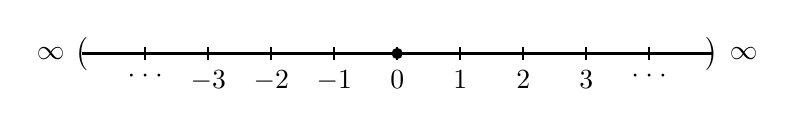
\begin{tikzpicture}[thick,scale=0.8, every node/.style={scale=1}]
        \draw[thick,-] (-5,0) -- (5,0);
        \foreach \x in {-3,-2,-1,0,1,2,3}
            \draw (\x cm,3pt) -- (\x cm,-3pt) node[anchor=north] {$\x$};
        \draw (-4 cm,3pt) -- (-4 cm,-3pt) node[anchor=north] {$\cdot\cdot\cdot$};
        \draw (4 cm,3pt) -- (4 cm,-3pt) node[anchor=north] {$\cdot\cdot\cdot$};
        \filldraw[black] (0,0) circle (2pt);
        \draw node[] at (-5,0) {$\big($};
        \draw node[] at (5,0) {$\big)$};
        \draw node[] at (-5.5,0) {$\infty$};
        \draw node[] at (5.5,0) {$\infty$};
    \end{tikzpicture}
    \caption{Representación del campo real con la recta real.} 
    \label{fig: Campo real}
\end{figure}


\textbf{El campo complejo}

\begin{tcolorbox}[breakable]
    
    \underline{Def.} El conjunto de los números complejos se define como
\[
\mathbb{C} := \{a+ib\mid a,b\in\mathbb{R}\}, \quad i := +\sqrt{-1}.
\]
\noindent Sea $z=a+ib$ un número complejo. Decimos que $a$ es su \emph{parte real} y que $b$ es su \emph{parte imaginaria}. A los números complejos con parte real nula, i.e., aquellos de la forma $0+ib, b\in\mathbb{R}$, se les conoce como números \emph{imaginarios}\footnote{Gauss prefería llamarles números \emph{laterales}, ya que creía que era un nombre más intuitivo, y que llamarles \emph{imaginarios} les dotaba de una opacidad misteriosa e innecesaria. Sugiero ver este video introductorio (o la serie completa, llamada \emph{Imaginary Numbers Are Real}) para perderles el miedo a los números imaginarios: \url{https://www.youtube.com/watch?v=T647CGsuOVU}.}. El \emph{complejo conjugado} de un número complejo de $z=a+ib$ es
\[
\overline{z} = a-ib,
\]
y el valor absoluto o \emph{módulo} de un número complejo $z$ es
\[
|z| = +\sqrt{z \overline{z}}.
\]
\end{tcolorbox}    

Apoyándonos en las operaciones del campo real, podemos definir la suma y multiplicación entre números complejos como\footnote{Nótese que la definición de multiplicación es igual al desarrollo de $(a+ib)(c+id)$ como producto de binomios.}.
\begin{align*}
    (a+ib)+(q+ir) &:=(a+q) + i(b+r), \\
    (a+ib)(q+ir)  &:= (aq-br) + i(ar+bq).
\end{align*}
 Así mismo, apoyándonos en el campo real, podemos comprobar que el conjunto $\mathbb{C}$ junto con estas dos operaciones forma un campo. 

\begin{ejer}\label{ejercicio-3}
    Prueba que $\mathbb{C}$, con las operaciones de suma y multiplicación definidas anteriormente, forma un campo.
\end{ejer}

% Geometría del campo complejo. Incluir en la descripción de la figura la nota al pie sobre los números \emph{laterales}\footnote{El mismísimo Gauss hubiera preferido este segundo nombre, ya que creía que era mucho más intuitivo, y que llamarlos \emph{imaginarios} les dotaba de una opacidad misteriosa e innecesaria. Sugiero ver este video introductorio (o la serie completa, llamada Imaginary Numbers Are Real) para perderles el miedo: \url{https://www.youtube.com/watch?v=T647CGsuOVU}.}

\subsubsection*{Subcampos} \label{Sssec: Subcampos}

\begin{tcolorbox}\label{Def: subcampo}
    
    \underline{Def.} Sea $(K,+,\cdot)$ un campo. Si $S\subseteq K$ es tal que las operaciones de suma y multiplicación en $K$ restringidas al dominio $S\times S$ forman un campo, decimos que $(S,+,\cdot)$ es un \emph{subcampo} de $(K,+,\cdot)$.
\end{tcolorbox}

\begin{Obs}\label{obs:1.4}
    \begin{enumerate}[label=(\arabic*)]\leavevmode
    
        \item Todo campo $K$ es trivialmente un subcampo de sí mismo.

        \item Si hacemos una identificación entre el conjunto de los números reales y los números complejos de la forma $a+i0\in\mathbb{C}, a\in\mathbb{R}$, entonces podemos considerar a $(\mathbb{R},+,\cdot)$ como un subcampo de $(\mathbb{C},+,\cdot)$. En efecto, si restringimos las operaciones de suma y multiplicación en el campo complejo al conjunto $\{z\in\mathbb{C}\mid z = a+i0, a\in\mathbb{R}\}$, entonces estas operaciones son idénticas a las operaciones de suma y multiplicación en el campo real.
    \end{enumerate}
\end{Obs}

Prácticamente todas las operaciones que realizamos cotidianamente como calcular fechas, dar cambio, aproximar áreas, repartir comida, etc., toman lugar en un campo. Es decir, las ideas intuitivas que nos formamos durante la educación básica de que la suma siempre debe ser conmutativa y asociativa \textemdash al igual que la multiplicación\textemdash, que existe la resta y la división, que el $0$ y el $1$ son números \emph{especiales} en cierto sentido y que siempre se cumple la propiedad de distributividad, son un \emph{hecho} para cualquier estructura de campo. Sin embargo, estas mismas ideas intuitivas \emph{no siempre se cumplen en otros tipos de estructuras algebraicas} \textemdash algunas de las cuales veremos más adelante\textemdash, \ ¡así que no te confíes!

\newpage
\subsection*{Espacios vectoriales} \label{Ssec: Espacios vectoriales}

El conjunto de soluciones de ciertos tipos de problemas que aparecen frecuentemente en varias áreas de las matemáticas, la física, la computación y la biomedicina tienen estructura de espacio vectorial, por lo que el conocimiento de la teoría de los espacios vectoriales \textemdash es decir, del álgebra lineal\textemdash \ se puede traducir en aplicaciones directas en dichas áreas. 

\subsubsection*{Definición de espacio vectorial} \label{Sssec: Definición de espacio vectorial}

\begin{tcolorbox}[breakable]
\underline{Def.} Un \emph{espacio vectorial} sobre un \hyperlink{Sssec: Definición de campo}{campo} $K$ es un conjunto $V$ con dos operaciones (llamadas \emph{adición} o \emph{suma vectorial} y \emph{producto de un vector por un escalar}) que satisfacen las siguientes propiedades, conocidas como los \emph{axiomas de los espacios vectoriales}:

\begin{center}
\begin{tabular}{lr}
    $\forall\hspace{1.5mm} \mathbf{u},\mathbf{v}\in V \hspace{3mm}\exists \hspace{1.5mm} \mathbf{u}+\mathbf{v}\in V$ & Cerradura de la adición \\ \\ \multirow{2}{0.4\textwidth}{$\forall\hspace{1.5mm} \mathbf{v}\in V, a\in K \hspace{3mm}\exists \hspace{1.5mm} a\mathbf{v}\in V$} & \multirow{2}{0.28\textwidth}{Cerradura del producto de un vector por un escalar} \\ \\ \\
    $\forall\hspace{1.5mm} \mathbf{u},\mathbf{v},\mathbf{w}\in V\hspace{3mm}\mathbf{u}+(\mathbf{v}+\mathbf{w})=(\mathbf{u}+\mathbf{v})+\mathbf{w}$  & Asociatividad de la adición\\ \\
    $\forall\hspace{1.5mm} \mathbf{u},\mathbf{v}\in V\hspace{3mm}\mathbf{u}+\mathbf{v}=\mathbf{v}+\mathbf{u}$ & Conmutatividad de la adición \\ \\
    $\exists \hspace{1.5mm} \mathbf{0}\in V$ t.q. $\mathbf{v}+\mathbf{0}=\mathbf{v}\hspace{3mm}\forall\hspace{1.5mm} \mathbf{v} \in V$ & Elemento identidad de la adición (neutro aditivo) \\ \\
    $\forall\hspace{1.5mm}\mathbf{v}\in V \hspace{3mm}\exists\hspace{1.5mm} -\mathbf{v}\in V$ t.q. $\mathbf{v}+(-\mathbf{v})=\mathbf{0}$ & Elemento inverso de la adición (inverso aditivo) \\ \\
    \multirow{2}{0.35\textwidth}{$a(b\mathbf{v})=(ab)\mathbf{v}\hspace{3mm}\forall a,b\in K, \mathbf{v}\in V$} & \multirow{2}{0.47\textwidth}{Compatibilidad del producto de un vector por un escalar con el producto entre escalares} \\ \\ \\
    \multirow{2}{0.4\textwidth}{$\exists\hspace{1.5mm}1\in K$ \hspace{1.5mm} t.q. $\hspace{1.5mm}1\mathbf{v}=\mathbf{v}\hspace{3mm}\forall\hspace{1.5mm} \mathbf{v}\in V$} & \multirow{2}{0.35\textwidth}{Elemento identidad del producto de un vector por un escalar} \\ \\ \\
    \multirow{2}{0.4\textwidth}{$a(\mathbf{v}+\mathbf{w})=a\mathbf{v}+a\mathbf{w}\hspace{3mm}\forall\hspace{1.5mm} \mathbf{v},\mathbf{w}\in V, a\in K$} & \multirow{2}{0.47\textwidth}{Distributividad del producto de un vector por un escalar con respecto a la adición vectorial}  \\ \\ \\
    \multirow{2}{0.4\textwidth}{$(a+b)\mathbf{v}=a\mathbf{v}+b\mathbf{v}\hspace{3mm}\forall\hspace{1.5mm} a,b\in K, \mathbf{v}\in V$} & \multirow{2}{0.47\textwidth}{Distributividad del producto de un vector por un escalar con respecto a la suma escalar.} \\ \\
\end{tabular}
\end{center}

A los elementos $a,b \in K$ del campo utilizado para definir el espacio vectorial se les llama \emph{escalares}, a los elementos $\mathbf{u},\mathbf{v},\mathbf{w}\in V$ que cumplen todas las propiedades anteriores se les llama \emph{vectores}, y el conjunto $V$ es llamado \emph{conjunto vectorial}.

\end{tcolorbox}

\begin{Obs}\label{obs:1.5}\leavevmode
 \begin{enumerate}[label=(\arabic*)]

    \item La definición matemática de \emph{vectores} como \emph{elementos cualesquiera de un conjunto V que, junto con un campo $K$ y las operaciones $+:V\times V\to V$ (suma vectorial) y $\ \cdot:K\times V\to V$ (producto de un vector por un escalar), cumplen las propiedades de un espacio vectorial} es muy distinta a la definición de vector como \emph{elemento con magnitud, dirección y sentido (y, más precisamente, que además es invariante bajo rotaciones propias e impropias)} utilizada en algunas áreas de la física, siendo la primera definición más general.

    \item La definición de \emph{espacio vectorial} incluye dos operaciones \emph{nuevas} (con respecto a las operaciones de campo) con una importante diferencia entre ellas: una es sólamente entre los elementos del conjunto $V$ (suma vectorial) y, la otra, entre los elementos del conjunto $V$ y el campo $K$ (producto de un vector por un escalar). Sin embargo, \emph{ambas dan como resultado un vector en $V$}.

    \item Así como la definición de \emph{campo} incluye un conjunto $K$ con dos operaciones (suma y producto) entre sus elementos que cumplen propiedades específicas, la definición de \emph{espacio vectorial} incluye un conjunto $V$ y un campo $K$ con dos operaciones (suma vectorial y producto de un vector por un escalar) entre sus elementos que cumplen propiedades específicas.
\end{enumerate}
\end{Obs}

\noindent Denotaremos a un espacio vectorial formado por un conjunto de vectores $V$ y un campo $K$ como $(V,K)$, o simplemente $V$ cuando sea claro sobre qué campo está definido. Más adelante veremos otras operaciones en espacios vectoriales que se pueden definir entre vectores y escalares; sin embargo, la suma vectorial y el producto de un vector por un escalar son las únicas necesarias para \emph{definir} a los espacios vectoriales, por lo que nos referiremos a ellas como las operaciones \emph{esenciales} de los espacios vectoriales.

\begin{Coro}[Ley de Cancelación para espacios vectoriales]\label{coro:1.6}
Sean $V$ un espacio vectorial y $\mathbf{x},\mathbf{y},\mathbf{z}\in V$ tales que $\mathbf{x}+\mathbf{z}=\mathbf{y}+\mathbf{z}$. Entonces, $\mathbf{x}=\mathbf{y}$.

\begin{proof}

    Se sigue la Ley de Cancelación (inciso (c) de la Proposición \ref{prop:1.2}) ya que, por definición de espacio vectorial, la suma vectorial es asociativa y todos los elementos de $V$ tienen elementos inversos bajo esta operación. Más aún, dado que la suma vectorial es conmutativa, se sigue que $\mathbf{x}+\mathbf{z} = \mathbf{z}+\mathbf{y}$ implica que $\mathbf{x}=\mathbf{y}$.
\end{proof}
\end{Coro}

Para complementar la discusión al respecto de qué es un vector y apreciar cómo funcionan las operaciones de los espacios vectoriales (suma vectorial y producto de un vector por un escalar) de manera visual, sugiero ver el siguiente video: \url{https://www.youtube.com/watch?v=fNk_zzaMoSs}.

\subsubsection*{Ejemplos de espacios vectoriales} \label{Ejem:Espacios_vectoriales}

Los ejemplos de espacios vectoriales más sencillos \textemdash y, a menudo, más útiles\textemdash \ se siguen de una muy importante relación existente entre las definiciones de campo y espacio vectorial.

\begin{ejer}\label{ejer-4}
    
    Sea $(K,+,\cdot)$ un campo. Demuestra que $(K,K)$ forma un espacio vectorial, con las operaciones de suma vectorial y producto de un vector por un escalar dadas por la suma y la multiplicación en el campo, respectivamente.
\end{ejer}

Por el Ejercicio \ref{ejer-4} tenemos que cualquier campo forma un espacio vectorial sobre sí mismo. En particular, $(\mathbb{R},\mathbb{R})$ y $(\mathbb{C},\mathbb{C})$ son espacios vectoriales. \\ % Este resultado se puede generalizar como sigue.

%\begin{ejer}\label{ejer-5}
%    
%    Sea $(S,+,\cdot)$ un subcampo de $(K,+,\cdot)$. Demuestra que $(K,S)$ forma un espacio vectorial.
%\end{ejer}

%Por el Ejercicio \ref{ejer-5} tenemos que un campo forma un espacio vectorial sobre cualquiera de sus subcampos. En particular, $(\mathbb{C},\mathbb{R})$ es un espacio vectorial. \\

Consideremos el conjunto $\mathbb{R}^2$. Aprovechando las operaciones de suma y multiplicación en el campo real, podemos definir una operación $+:\mathbb{R}^2\times\mathbb{R}^2\to \mathbb{R}^2$ como
\[
    (x_1, x_2) + (y_1,y_2) := (x_1+y_1,x_2+y_2)
\] 
y una operación $\cdot:\mathbb{R}\times \mathbb{R}^2\to \mathbb{R}^2$ como
\[
    a(x_1,x_2) := (ax_1,ax_2).
\] 
Se puede verificar que, con estas operaciones, $\mathbb{R}^2$ forma un espacio vectorial sobre el campo real, en el cual el neutro aditivo es $(0,0)\in\mathbb{R}^2$ y el inverso aditivo de $(x_1,x_2)\in\mathbb{R}^2$ es $(-x_1,-x_2)\in\mathbb{R}^2$. Esto se debe a que definimos las nuevas operaciones ``entrada por entrada'', por lo que la demostración de que $(\mathbb{R}^2,\mathbb{R})$ es un espacio vectorial es análoga a la del Ejercicio \ref{ejer-4}. Más aún, para cualquier entero positivo $n$ podemos definir operaciones $+:\mathbb{R}^n\times \mathbb{R}^n\to \mathbb{R}^n$ y $\cdot:\mathbb{R}\times \mathbb{R}^n\to \mathbb{R}^n$ de manera análoga a las anteriores, obteniendo así un espacio vectorial $(\mathbb{R}^n,\mathbb{R})$. Por ende, tenemos el siguiente corolario del Ejercicio \ref{ejer-4}.

\begin{Coro}\label{coro:1.7}
    
    Sean $K$ un campo y $n$ un entero positivo. Entonces $(K^n,K)$ es un espacio vectorial, definiendo las operaciones de suma vectorial y producto de un vector por un escalar entrada por entrada.
\end{Coro}

\noindent Por el Corolario \ref{coro:1.7}, se sigue que $(\mathbb{C}^n,\mathbb{C})$ es un espacio vectorial para cualquier entero positivo $n$. Ahora, veamos otros ejemplos de espacios vectoriales. \\

El conjunto de todas las funciones polinomiales de una variable real de grado $n$ (i.e., con regla de correspondencia de la forma $f(x) = c_1 x^1 + c_2 x^2 + ... + c_n x^n, \hspace{1.5mm} c_i \in \mathbb{R}, \hspace{1.5mm} i \in \{1,2,...,n\}$) y con un mismo dominio $\mathcal{D}$ forma un espacio vectorial sobre el campo real. Aquí, las definiciones de suma vectorial y de producto de un vector por un escalar se siguen naturalmente de la definición de la suma de funciones $(f+g)(x):= f(x)+g(x)$ y del producto de una función arbitraria $f(x)$ por una función constante $a$, respectivamente, vistas en cálculo \textemdash las cuales aplican para las intersecciones de los dominios. El elemento identidad de la suma vectorial (neutro aditivo) es la función constante cero $f(x)=0\hspace{2.5mm} \forall\hspace{0.5mm}x\in\mathcal{D}$ y el inverso aditivo de una función $g(x)$ es $-g(x)$. Observemos que, en este caso, los \emph{vectores} de nuestro espacio vectorial \emph{son funciones} (en particular, en este ejemplo, son funciones polinomiales). \\

El conjunto de todas las funciones de una variable real derivables y con derivada continua (i.e., funciones de clase $C^1$) sobre el campo real forma un espacio vectorial\footnote{En general, el conjunto de funciones de clase $C^n$ sobre el campo $\mathbb{R}$ forma un espacio vectorial; aunque, estrictamente hablando, $C^1$ y $C^n$ son \emph{clases} y no conjuntos, en este curso ignoraremos este tecnicismo.}. Esto probablemente lo viste de manera implícita en tu curso de cálculo diferencial de una variable, cuando viste los teoremas de derivadas de una suma/multiplicación/división de funciones (también conocido como \emph{álgebra de derivadas}) para funciones de este tipo. Las operaciones en este espacio vectorial, así como los elementos identidad (neutros) e inversos, se definen de la misma forma que en el ejemplo de las funciones polinomiales. \\

Para futura referencia, dejamos la siguiente definición.

\begin{tcolorbox}
    \underline{Def.} Un \emph{espacio vectorial real (complejo)} es aquel definido sobre el campo real (complejo) o, equivalentemente, aquel donde los escalares son números reales (complejos).
\end{tcolorbox}{}

Para ver más ejemplos de espacios vectoriales pueden consultar, por ejemplo, \emph{Linear Algebra} de Friedberg (págs. 8-11.) o \emph{Linear Algebra: A Modern Introduction} de Poole (págs. 430-432), entre otros. \\

\begin{Teo}\label{teo:1.8}
    Sea ($V$,$K$) un espacio vectorial arbitrario con $\mathbf{v}\in V$ y $a\in K$. Entonces, tenemos que:
    \begin{enumerate}[label=(\alph*)]

        \item $0\mathbf{v}=\mathbf{0}$;

        \item $a\mathbf{0}=\mathbf{0}$;

        \item $(-a)\mathbf{v}=-(a\mathbf{v})=a(-\mathbf{v})$.
    \end{enumerate}
\end{Teo}

\begin{proof}\leavevmode
    \begin{enumerate}[label=(\alph*)]

        \item Por la propiedad de cerradura del producto de un vector por un escalar, sabemos que $0\mathbf{v}\in V$. Ahora, observemos que
            \begin{align*}
                0\mathbf{v}+0\mathbf{v}&=(0+0)\mathbf{v} \tag{distributividad} \\
                                       &=0\mathbf{v} \\
                                       &=0\mathbf{v}+\mathbf{0} \tag{neutro aditivo},
            \end{align*}
            donde la primera igualdad se sigue de la distributividad de la suma de escalares con respecto al producto de un vector por un escalar. Por ende, tenemos que $0\mathbf{v}+0\mathbf{v} =0\mathbf{v}+\mathbf{0}$. Luego, de la Ley de Cancelación para espacios vectoriales (Corolario \ref{coro:1.6}) se sigue que $0\mathbf{v}=\mathbf{0}$.

        \item Observemos que
            \begin{align*}
                a\mathbf{0}+a\mathbf{0}&=a(\mathbf{0}+\mathbf{0}) \\
                                       &=a\mathbf{0}\\
                                       &=a\mathbf{0}+\mathbf{0},
            \end{align*}
            donde la primera igualdad se sigue de la distributividad de la suma vectorial con respecto al producto de un vector por un escalar. Por ende, tenemos que $a\mathbf{0}+a0\mathbf{}=a\mathbf{0}+\mathbf{0}$. Luego, de la Ley de Cancelación para espacios vectoriales (Corolario \ref{coro:1.6}) se sigue que $a\mathbf{0}=\mathbf{0}$.

        \item Observemos que
            \begin{align*}
                \mathbf{0} &= 0\mathbf{v} \\
                           &= (a+(-a)) \mathbf{v} \\
                           &= a\mathbf{v} + (-a)\mathbf{v},
            \end{align*}
            donde se utilizó el inciso (a), la propiedad de existencia de inversos aditivos en un campo y la distributividad de la suma de escalares con respecto al producto de un vector por un escalar. De la ecuación $a\mathbf{v} + (-a)\mathbf{v} = \mathbf{0}$ y la conmutatividad de la suma vectorial se sigue que $(-a)\mathbf{v} = -(a\mathbf{v})$. Análogamente, tenemos que
            \begin{align*}
                \mathbf{0} &= a\mathbf{0} \\
                           &= a(\mathbf{v} + (-\mathbf{v})) \\
                           &= a\mathbf{v} + a(-\mathbf{v}),
            \end{align*}
            donde se utilizó el inciso (b), la propiedad de existencia de inversos aditivos en un espacio vectorial y la distributividad de el producto de un vector por un escalar con respecto a la suma vectorial. De la ecuación $a\mathbf{v}+a(-\mathbf{v}) = \mathbf{0}$ y la conmutatividad de la suma vectorial se sigue que $a(-\mathbf{v}) = -(a\mathbf{v})$. Por ende, $(-a)\mathbf{v} = -(a\mathbf{v}) = a(-\mathbf{v})$..

    \end{enumerate}
\end{proof}

\subsubsection*{Interpretación geométrica de las operaciones esenciales de los espacios vectoriales} \label{Sssec:Interpretación geométrica de las operaciones de los espacios vectoriales}

Como se mencionó en una nota al final de la sección \ref{Ejem:Espacios_vectoriales} \hspace{1.5mm}\textemdash de la cual retomaremos muchas ideas a continuación\textemdash, podemos desarrollar nuestra intuición sobre muchos temas del álgebra lineal trabajando en espacios vectoriales \emph{visualizables}, para luego extenderla a espacios vectoriales más generales. Por ende, ahora haremos hincapié en la interpretacción geométrica de las operaciones de suma vectorial y producto de un vector por un escalar en el espacio vectorial real $\mathbb{R}^2$, así como en el espacio vectorial complejo $\mathbb{C}$.


\subsubsection*{El espacio vectorial real \texorpdfstring{$\mathbb{R}^2$}{TEXT}} \label{Sssec: El espacio vectorial real R^2}

En geometría analítica aprendimos que, con la ayuda de un sistema de coordenadas, podemos formar una correspondencia uno a uno (o \emph{biunívoca}) entre pares ordenados $(a,b)$ con entradas reales\footnote{Es decir, con $a,b\in\mathbb{R}$.} y puntos del plano cartesiano $\mathbb{R}\times\mathbb{R}$. En particular, si tomamos el sistema de coordenadas cartesianas, entonces a cualquier par ordenado de entradas reales $(a,b)$ le corresponde un punto en el plano cartesiano $\mathbb{R}\times\mathbb{R}$ con coordenadas cartesianas $(a,b)$, y vice versa. En álgebra lineal, es preferible considerar a cada vector $(a,b)\in\mathbb{R}^2$ en una correspondencia biunívoca con la flecha en el plano cartesiano que tiene cola en el origen y punta en la coordenada cartesiana correspondiente al punto $(a,b)$, como se muestra en la Figura \ref{fig:Correspondencias_del_plano_cartesiano}. \\

\begin{figure}[h!]
    \centering
    \begin{tikzpicture}[thick,scale=0.8, every node/.style={scale=1}]
        \draw[thick,<->] (-4,0) -- (4,0);
        \draw[thick,<->] (0,-4) -- (0,4);
        \draw[step=1cm,gray,very thin,dashed] (-3.9,-3.9) grid (3.9,3.9);
        \foreach \x in {1,2,3}
            \draw (\x cm,1pt) -- (\x cm,-1pt) node[anchor=north] {$\x$};
        \foreach \y in {1,2,3}
            \draw (1pt,\y cm) -- (-1pt,\y cm) node[anchor=east] {$\y$};
        \foreach \x in {-3,-2,-1}
            \draw (\x cm, 1pt) -- (\x cm, -1pt);
        \foreach \y in {-3,-2,-1}
            \draw (1pt,\y cm) -- (-1pt,\y cm);
        \filldraw[black] (0,0) circle (2pt) node[] at (-0.6,0.35) {\small{$(0,0)$}};
        \draw[ROJO,very thick,->] (0,0) -- (2,3) node[] at (3,2.5) {$(2,3)$};
        \draw[AZUL,very thick,->] (0,0) -- (-3.5,-2) node[] at (-2,-2.5) {$(-3.5,-2)$};
    \end{tikzpicture}
    \caption{Ejemplo de representación de vectores en el plano cartesiano. Los vectores $(-3.5,-2)$ y $(2,3)$ son representados por flechas que tienen su cola en el origen del plano cartesiano y su punta en las coordenadas correspondientes.}
    \label{fig:Correspondencias_del_plano_cartesiano}
\end{figure}

\textbf{Suma vectorial} \\

Recordemos que, en este espacio, la suma vectorial se define como $(a,b)+(c,d)=(a+c,b+d)$, i.e., entrada por entrada. Podemos calcular, por ejemplo, la suma $(2,1)+(1,3) = (3,4)$. Los tres vectores mencionados se muestran en la Figura \ref{fig:Suma_vectorial}.

\begin{figure}[h!]
    \centering
    \begin{tikzpicture}[thick,scale=1.6, every node/.style={scale=1}]
        \draw[thick,->] (0,0) -- (4.5,0);
        \draw[thick,->] (0,0) -- (0,4.5);
        \draw[step=1cm,gray,thin,dashed] (0,0) grid (4.4,4.4);
        \foreach \x in {0,1,2,3,4}
            \draw (\x cm,1pt) -- (\x cm, -1pt) node[anchor=north] {$\x$};
        \foreach \y in {1,2,3,4}
            \draw (1pt,\y cm) -- (-1pt,\y cm) node[anchor=east] {$\y$};
        
            \draw[ROJO,very thick,->] (0,0) -- (2,1) node[] at (2.05,0.5){$(2,1)$};
            \draw[AZUL,very thick,->] (0,0) -- (1,3) node[] at (0.55,3) {$(1,3)$};
            \draw[violet,very thick,->] (0,0) -- (3,4) node[] at (3,4.2) {$(3,4)$};
            \draw[] node[] at (4.2,4.2) {\textbf{a)}};
            \draw[black,thick,->]  (5,2) -- (5.5,2);
    \end{tikzpicture} \hspace{0.5cm} \begin{tikzpicture}[thick,scale=1.6, every node/.style={scale=1}]
        \draw[thick,->] (0,0) -- (4.5,0);
        \draw[thick,->] (0,0) -- (0,4.5);
        \draw[step=1cm,gray,thin,dashed] (0,0) grid (4.4,4.4);
        \foreach \x in {0,1,2,3,4}
            \draw (\x cm,1pt) -- (\x cm, -1pt) node[anchor=north] {$\x$};
        \foreach \y in {1,2,3,4}
            \draw (1pt,\y cm) -- (-1pt,\y cm) node[anchor=east] {$\y$};
            \draw[ROJO,very thick,->] (0,0) -- (2,1) node[] at (2.05,0.5){$(2,1)$};
            \draw[AZUL,dashed,->] (2,1) -- (3,4);
            \draw[AZUL,very thick,->] (0,0) -- (1,3) node[] at (0.55,3) {$(1,3)$};
            \draw[ROJO,dashed,->] (1,3) -- (3,4);
            \draw[violet,very thick,->] (0,0) -- (3,4) node[] at (3,4.2) {$(3,4)$};
            \draw[] node[] at (4.2,4.2) {\textbf{b)}};
    \end{tikzpicture}
    \caption{Interpretación geométrica de la suma vectorial en el espacio vectorial real $\protect\mathbb{R}^2$. En la subfigura $\textbf{a)}$ se observan los vectores $(1,3)$ y $(2,1)$, así como el vector resultante de la suma de los dos anteriores, $(3,4)$. En la subfigura $\textbf{b)}$ observamos la llamada \emph{Ley del paralelogramo} para la suma de dos vectores.}
    \label{fig:Suma_vectorial}
\end{figure}

    Observemos que, visualmente, esto corresponde a trazar uno de los vectores en el plano cartesiano y luego trazar el otro colocando la cola en la punta del vector anterior, como si ése fuese su origen. Nótese que no importa cuál vector trazamos primero y cuál después, lo cual concuerda con la conmutatividad de la suma vectorial (esta misma interpretación geométrica es válida para la suma de tres o más vectores de $\mathbb{R}^2$: basta irlos sumando de dos en dos vectores); a esto se le conoce como la \emph{Ley del paralelogramo}. Es decir, la suma de dos vectores $\mathbf{u},\mathbf{v}\in\mathbb{R}^2$ es igual a la diagonal principal del paralelogramo formado por las flechas que los representan. %En particular, $\forall \ \mathbf{v} \in \mathbb{R}^2$, $\mathbf{0}+\mathbf{v}=\mathbf{v}$, lo cual concuerda con el hecho de que el vector $\mathbf{v}$ corresponda a una flecha con cola en el origen.

\begin{ejer}
    Muestra intuitivamente que si transportamos a la \emph{otra} diagonal del paralelogramo hasta el origen (lo cual se puede hacer de dos maneras distintas), obtenemos a las representaciones de los vectores $\mathbf{u}-\mathbf{v}$ y $\mathbf{v}-\mathbf{u}$. 
\end{ejer}

\textbf{Producto de un vector por un escalar} \\

Ahora, recordemos que en este espacio el producto de un vector por un escalar se define como $c(a,b) = (ca,cb)$ (entrada por entrada). Podemos calcular, por ejemplo, los productos $\big(\frac{1}{2}\big)(2,2)=(1,1)$ y $(-1.2)(1,3)=(-1.2,-3.6)$. La representación gráfica de estas operaciones se muestra en la Figura \ref{fig:Producto_de_un_vector_por_un_escalar}.

\begin{figure}[h!]
    \centering
    \begin{tikzpicture}[thick,scale=0.8, every node/.style={scale=1}]
        \draw[thick,<->] (-4,0) -- (4,0);
        \draw[thick,<->] (0,-4) -- (0,4);
        \draw[step=1cm,gray,thin,dashed] (-3.9,-3.9) grid (3.9,3.9);
        \foreach \x in {1,2,3,4}
            \draw (\x cm,1pt) -- (\x cm, -1pt) node[anchor=north] {$\x$};
        \foreach \y in {1,2,3,4}
            \draw (1pt,\y cm) -- (-1pt,\y cm) node[anchor=east] {$\y$};
            \draw[ROJO,very thick,->] (0,0) -- (2,2) node[anchor=west] {$(2,2)$};
            \draw[AZUL,very thick,->,opacity=0.7] (0,0) -- (1,3) node[anchor=south west] {$(1,3)$};
            \draw[black,thick,->]  (5,0) -- (5.7,0);
            \draw[] node[] at (3.5,3.5) {\textbf{a)}};
            \end{tikzpicture} \hspace{0.5mm} \begin{tikzpicture}[thick,scale=0.8, every node/.style={scale=1}]
        \draw[thick,<->] (-4,0) -- (4,0);
        \draw[thick,<->] (0,-4) -- (0,4);
        \draw[step=1cm,gray,thin,dashed] (-3.9,-3.9) grid (3.9,3.9);
        \foreach \x in {1,2,3,4}
            \draw (\x cm,1pt) -- (\x cm, -1pt) node[anchor=north] {$\x$};
        \foreach \y in {1,2,3,4}
            \draw (1pt,\y cm) -- (-1pt,\y cm) node[anchor=east] {$\y$};
            \draw[ROJO,very thick,opacity=0.7,->] (0,0) -- (1,1) node[] at (2.1,0.65) {$(1,1)$};
            \draw[AZUL,very thick,->] (0,0) -- (-1.2,-3.6) node[] at (-3,-3.4) {$(-1.2,-3.6)$};
            \draw[ROJO,thin,dashed,->] (0,0) -- (2,2); 
            \draw[AZUL,thin,dashed,->,opacity=0.7] (0,0) -- (1,3); 
            \draw[] node[] at (3.5,3.5) {\textbf{b)}};
    \end{tikzpicture}
    \caption{Interpretación geométrica del producto de un vector por un escalar en el espacio vectorial real $\mathbb{R}^2$. Comparando las subfiguras $\textbf{a)}$ y $\textbf{b)}$ observamos que, en caso de que se multiplique a un vector de $\mathbb{R}^2$ por un escalar de $\mathbb{R}$, es posible que la longtitud del vector cambie y que su sentido se invierta, pero su dirección no cambia.}
    \label{fig:Producto_de_un_vector_por_un_escalar}
\end{figure}


Como podemos observar, el primer producto redujo la longitud del vector sin cambiar su sentido, mientras que el segundo producto aumentó la longitud del vector, a la vez que invirtió su sentido; sin embargo, en ambos casos, el producto de un vector por un escalar no cambió la \emph{dirección} de los vectores\textemdash es decir, los mantuvo en la misma \emph{línea}. En general, si el escalar $c\in\mathbb{R}$ que multiplica al vector tiene $|c|>1$, lo \emph{alarga}; si tiene $|c|<1$, lo acorta; finalmente, si tiene $|c|=1$, no cambia su longitud. Por este cambio de longitud es que al producto de un vector por un escalar también se le conoce por el nombre \emph{reescalamiento}. Además, si $c>0$, el vector mantiene su misma dirección y sentido (sigue en la misma línea y apunta hacia el mismo lado) mientras que, si $c<0$, el vector conserva su dirección pero se invierte su sentido (sigue en la misma línea pero apunta hacia el lado opuesto); si $c=0$ entonces el vector automáticamente se convierte en el vector nulo $(0,0)$, como se demostró algebráicamente en el inciso (a) del Teorema \ref{teo:1.8}. Para visualizar las operaciones de adición vectorial y producto de un vector por un escalar de forma interactiva, recomiendo la sección \textbf{Vector Algebra and Geometry} de \url{https://textbooks.math.gatech.edu/ila/vectors.html}, así como la ilustración interactiva \url{http://immersivemath.com/ila/ch02_vectors/ch02.html#fig_vec_scaling}. \\

    Así, en general, si combinamos las operaciones de suma vectorial y producto de un vector por un escalar, visualmente lo que estaremos haciendo será \emph{combinar líneas} con diferentes longitudes, direcciones y sentidos en el plano cartesiano. \\

Nota: El vector nulo $\mathbf{0}=(0,0)$ (también llamado \emph{vector origen}) no tiene longitud, ya que es el único donde la cola y la punta de su flecha coinciden. Además, tampoco tiene dirección ni sentido\footnote{Alternativamente, se dice que tiene \emph{todas las direcciones} y \emph{todos los sentidos simultáneamente}: en la práctica, ambas interpretaciones son equivalentes, pero la primera puede ser más fácil de asimilar.}. Si asumimos que este vector no tiene longitud, dirección ni sentido, entonces queda claro por qué cualquier reescalamiento de este vector no lo modifica, como se demostró en el inciso (b) del Teorema \ref{teo:1.8}.

\begin{ejer}
    Interpreta geométricamente las operaciones esenciales del espacio vectorial $\mathbb{R}^3$.
\end{ejer}

\subsubsection*{En el espacio vectorial complejo \texorpdfstring{$\mathbb{C}$}{TEXT}}

Como hemos visto, el plano cartesiano nos sirve para representar vectores con dos entradas reales. De manera similar, el \emph{plano complejo} \textemdash con un eje de números \emph{reales} (por convención, el horizontal) y otro eje perpendicular a él de números \emph{imaginarios}\footnote{Los números imaginarios son aquellos números complejos con la parte real igual a cero, i.e. $0+ib=ib\in\mathbb{C}$, donde $b$ es un número real. En otras palabras, son el resultado de multiplicar el número imaginario $i$ por cualquier número real.}\textemdash\hspace{0.5mm} nos sirve para representar vectores con una entrada compleja. Así, cada vector de una entrada compleja $\begin{pmatrix}a+ib\end{pmatrix}$ con $a,b\in\mathbb{R}$ tiene una correspondencia uno a uno con una flecha con cola en el origen del plano y flecha en la coordenada $(a,b)$ del plano complejo, la cual corresponde a, desde el origen, moverse $a$ unidades sobre el eje real y $b$ unidades sobre el eje imaginario. \\

\textbf{Suma vectorial} \\

De la definición de suma vectorial $\begin{pmatrix}a+ib\end{pmatrix}+\begin{pmatrix}c+id\end{pmatrix}:=\begin{pmatrix}(a+c)+(b+d)i\end{pmatrix}$ se deduce que la suma vectorial entre vectores de $\mathbb{C}$ tiene la misma interpretación geométrica que aquella entre vectores de $\mathbb{R}^2$. Por ejemplo, si calculamos $\begin{pmatrix}1+2i\end{pmatrix}+\begin{pmatrix}3+2i\end{pmatrix}=\begin{pmatrix}4+4i\end{pmatrix}$, podemos representarlo visualmente en la Figura \ref{fig:Suma_vectorial_compleja}. \\

\begin{figure}[h!]
    \centering
    \begin{tikzpicture}
        \draw[thick,->] (0,0) -- (5,0);
        \draw[thick,->] (0,0) -- (0,5);
        \draw[step=1cm,gray,thin,dashed] (0,0) grid (4.9,4.9);
        \foreach \x in {1,2,3,4}
            \draw (\x cm,1pt) -- (\x cm, -1pt) node[anchor=north] {$\x$};
        \draw (1pt, 1cm) -- (-1pt, 1 cm) node[anchor=east] {$i$};
        \foreach \y in {2,3,4}
            \draw (1pt,\y cm) -- (-1pt,\y cm) node[anchor=east] {$\y i$};
            \draw[AZUL,very thick,->] (0,0) -- (1,2) node[] at (0.8,2.6) {$\begin{pmatrix} 1 + 2i \end{pmatrix}$};
            \draw[ROJO,thin,dashed,->] (1,2) -- (4,4) node[] at (2.4,3.8) {$\begin{pmatrix} 3 + 2i \end{pmatrix}$};
            \draw[ROJO,very thick,->] (0,0) -- (3,2) node[] at (3.1,1.2) {$\begin{pmatrix} 3 + 2i \end{pmatrix}$};
            \draw[AZUL,thin,dashed,->] (3,2) -- (4,4) node[] at (4.2,2.6) {$\begin{pmatrix} 1 + 2i \end{pmatrix}$};
        \draw[violet,very thick,->] (0,0) -- (4,4) node[anchor=south west] {$\begin{pmatrix} 4 + 4i \end{pmatrix}$};
    \end{tikzpicture}
    \caption{Interpretación geométrica de la suma vectorial en el espacio vectorial complejo $\mathbb{C}$. Observamos que, al igual que en el caso del espacio vectorial real $\mathbb{R}^2$, se cumple la \emph{Ley del paralelogramo}.}
    \label{fig:Suma_vectorial_compleja}
\end{figure}

\textbf{Producto de un vector por un escalar} \\

Por definición, el producto de un vector por un escalar es $(q+ir)\begin{pmatrix}s+it\end{pmatrix}:=\begin{pmatrix}(qs-rt)+i(qt+rs)\end{pmatrix}$. Notemos que, en particular, si la parte imaginaria del escalar es nula (i.e., si $r=0$), entonces el escalar es un número real y el producto resultante es $(q)\begin{pmatrix}s+it\end{pmatrix}:=\begin{pmatrix}(qs)+(qt)i\end{pmatrix}$, por lo cual geométricamente sólo se produce un reescalamiento totalmente análogo al discutido en el caso de $\mathbb{R}^2$. En cambio, ahora observemos qué sucede si la parte real del escalar es nula y la parte imaginaria es igual a $1$ (i.e., si multiplicamos por el escalar $i$). Tomemos, por ejemplo, al vector $\begin{pmatrix}2+2i\end{pmatrix}$. Al hacer el producto de este vector por $i$ obtenemos $\begin{pmatrix}-2+2i\end{pmatrix}$. Si, en cambio, hacemos el producto de este mismo vector por el escalar $-i$, obtenemos como resultado $(-i)\begin{pmatrix}2+2i\end{pmatrix}=\begin{pmatrix}2-2i\end{pmatrix}$. Ambas operaciones se muestran de manera visual en la Figura \ref{fig:Producto_de_un_vector_complejo_por_i}. \\

\begin{figure}[h!]
    \centering
    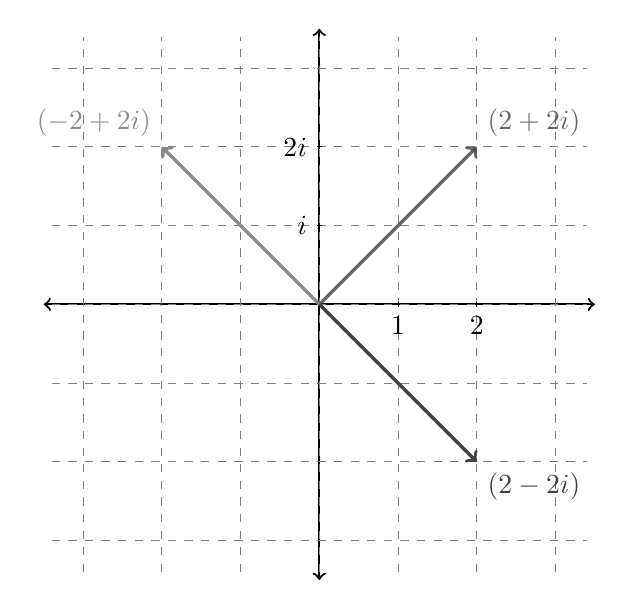
\begin{tikzpicture}
        \draw[thick,<->] (-3.5,0) -- (3.5,0);
        \draw[thick,<->] (0,-3.5) -- (0,3.5);
        \draw[step=1cm,gray,thin,dashed] (-3.4,-3.4) grid (3.4,3.4);
        \foreach \x in {1,2}
            \draw (\x cm,1pt) -- (\x cm, -1pt) node[anchor=north] {$\x$};
            \draw (1pt,1 cm) -- (-1pt,1 cm) node[anchor=east] {$i$};
            \draw (1pt,2 cm) -- (-1pt,2 cm) node[anchor=east] {$2i$};
            \draw[darkgray,very thick,opacity=0.8,->] (0,0) -- (2,2) node[anchor=south west] {$(2+2i)$};
            \draw[gray,very thick,opacity=0.9,->] (0,0) -- (-2,2) node[anchor=south east] {$(-2+2i)$};
            \draw[darkgray,very thick,->] (0,0) -- (2,-2) node[anchor=north west] {$(2-2i)$};
    \end{tikzpicture}
    \caption{Interpretación geométrica del producto de un vector complejo por los números imaginarios $i$ y $-i$. En este caso, nuestro vector base es $(2+2i)$. El producto de este vector por el escalar $i$ resulta en el vector $(-2+2i)$, lo cual puede ser interpretado geométricamente como una rotación discreta de $\frac{\pi}{2}$ radianes. Así observamos que, en cambio, el producto de nuestro vector base $(2+2i)$ por $-i$ se puede interpretar geométricamente como una rotación discreta de $-\frac{\pi}{2}$ radianes.}
    \label{fig:Producto_de_un_vector_complejo_por_i}
\end{figure}

   Aquí vemos que hacer el producto de un vector por el escalar $i$ \emph{equivale a hacer una rotación de $90^\circ$ ó $\frac{\pi}{2}$ radianes}. Análogamente, el producto de un vector por el escalar $-i$ equivale a hacer una rotación de $-90^\circ$ ó $-\frac{\pi}{2}$ radianes. Esto tiene sentido ya que $-i=-1(i)=i(-1)$ lo cual implica que, debido a la compatibilidad del producto de un vector por un escalar con el producto entre escalares, es lo mismo multiplicar un vector por $(-i)$ a multiplicarlo por $i$ y después por -1, o vice versa: el razonamiento geométrico correspondiente es que da lo mismo rotar un vector $-\frac{\pi}{2}$ radianes a rotarlo $\frac{\pi}{2}$ radianes y después invertir su sentido, o primero invertir su sentido y después rotarlo $\frac{\pi}{2}$ radianes. \\

   ¿Y si multiplicamos un vector de $\mathbb{C}$ por un escalar $ai$ con $a\neq 0,1$? Ya que $ai\begin{pmatrix}b + ic\end{pmatrix}=\begin{pmatrix}-ac+i(ab)\end{pmatrix}=a\begin{pmatrix}-c+ib\end{pmatrix}=a(i\begin{pmatrix}b+ic\end{pmatrix})$ \textemdash es decir, por la compatibilidad entre productos\textemdash\hspace{0.5mm} podemos deducir que hacer el producto de un vector complejo por un número imaginario arbitrario $ai$ tendrá dos consecuencias: rotarlo de acuerdo a $i$ ($\frac{\pi}{2}$ radianes a contrarreloj) y reescalarlo de acuerdo al valor de $a$ (invirtiendo el sentido si $a<0$). En este último caso, ya que $ai=|a|(-i)=(-i)|a| \ \ \forall \ a<0$, también podríamos pensar que se rota al vector complejo de acuerdo a $-i$ ($\frac{\pi}{2}$ radianes en el sentido de las manecillas) y se reescala de acuerdo al valor absoluto de $a$: ¡ambas interpretaciones son equivalentes! \\

   Dicho lo anterior, estamos listos para el caso más general, el cual es fácil de entender de forma precisa recordando la representación polar de los números complejos. Sea $z=x+iy\in\mathbb{C}$. Entonces sus coordenadas cartesianas en el plano complejo son $(x,y)$, mientras que sus coordenadas polares son $(r,\theta)$, donde $x=r\cos\theta, y = r\sin\theta$. Observemos que $r = +\sqrt{x^2+y^2} = +\sqrt{(x+iy)(x-iy)} = +\sqrt{z \overline{z}} = |z|$, por lo que el \emph{módulo} de $z$ es igual a la longitud de la flecha que representa a $z$ en el plano complejo. Por otro lado, $\theta$ es el ángulo que va de la parte positiva del eje real a la flecha que representa a $z$ en el plano y se conoce como el \emph{argumento} de $z$. Por ende, tenemos que
   \begin{align*}
       z &= x+iy \\
         &= |z|\cos\theta + i|z|\sin\theta \\
         &= |z|(\cos\theta+i\sin\theta)
   \end{align*}
   para todo $z\in\mathbb{C}$. Sean $z_1,z_2\in\mathbb{C}$ con argumentos $\theta_1$ y $\theta_2$, respectivamente. Entonces, por lo anterior,
   \begin{align*}
       z_1z_2 &= |z_1|(\cos\theta_1+i\sin\theta_1)|z_2|(\cos\theta_2+i\sin\theta_2) \\
              &= |z_1||z_2|(\cos\theta_1\cos\theta_2 +i\cos\theta_1\sin\theta_2 + i\sin\theta_1\cos\theta_2-\sin\theta_1\sin\theta_2) \\
              &= |z_1||z_2|\big(\cos\theta_1\cos\theta_2 -\sin\theta_1\sin\theta_2 + i(\cos\theta_1\sin\theta_2+\cos\theta_2\sin\theta_1)\big).
   \end{align*}
   Luego, aplicando las identidades trigonométricas para el coseno y seno de una suma de ángulos
   \begin{align*}
       \cos(\alpha+\beta) &= \cos(\alpha)\cos(\beta)-\sin(\alpha)\sin(\beta), \\
       \sin(\alpha+\beta) &= \cos\alpha\sin\beta + \cos\beta\sin\alpha,
   \end{align*}
   tenemos que
   \[
   z_1z_2 = |z_1||z_2|(\cos(\theta_1+\theta_2) + i\sin(\theta_1+\theta_2)).
   \] 
   Por lo tanto, el producto de dos números complejos se obtiene \emph{multiplicando sus módulos} y \emph{sumando sus argumentos}. \\

   Ya que el producto de un vector por un escalar en $(\mathbb{C},\mathbb{C})$ es igual al producto entre escalares complejos, concluimos que multiplicar un vector complejo $(s+it)$ por un escalar complejo $q+ir$ con $q,r\neq0$ reescalará el vector $(s+it)$ en el plano complejo por el módulo de $q+ir$ y lo rotará de acuerdo al argumento de $q+ir$. En general, en los espacios vectoriales complejos los escalares no sólamente pueden \emph{reescalar} vectores, sino que también los pueden \emph{rotar}. 
\end{document}
